\documentclass[main.tex]{subfiles}

\begin{document}
This is the homework from problem set 1. This document was generated using
\LaTeX. If you have any questions feel free to contact me at nharvey@spsu.edu.

\begin{enumerate}
	\setcounter{enumi}{10}
	\item 
		\begin{minipage}[H]{\textwidth}
			\vspace{0pt}
			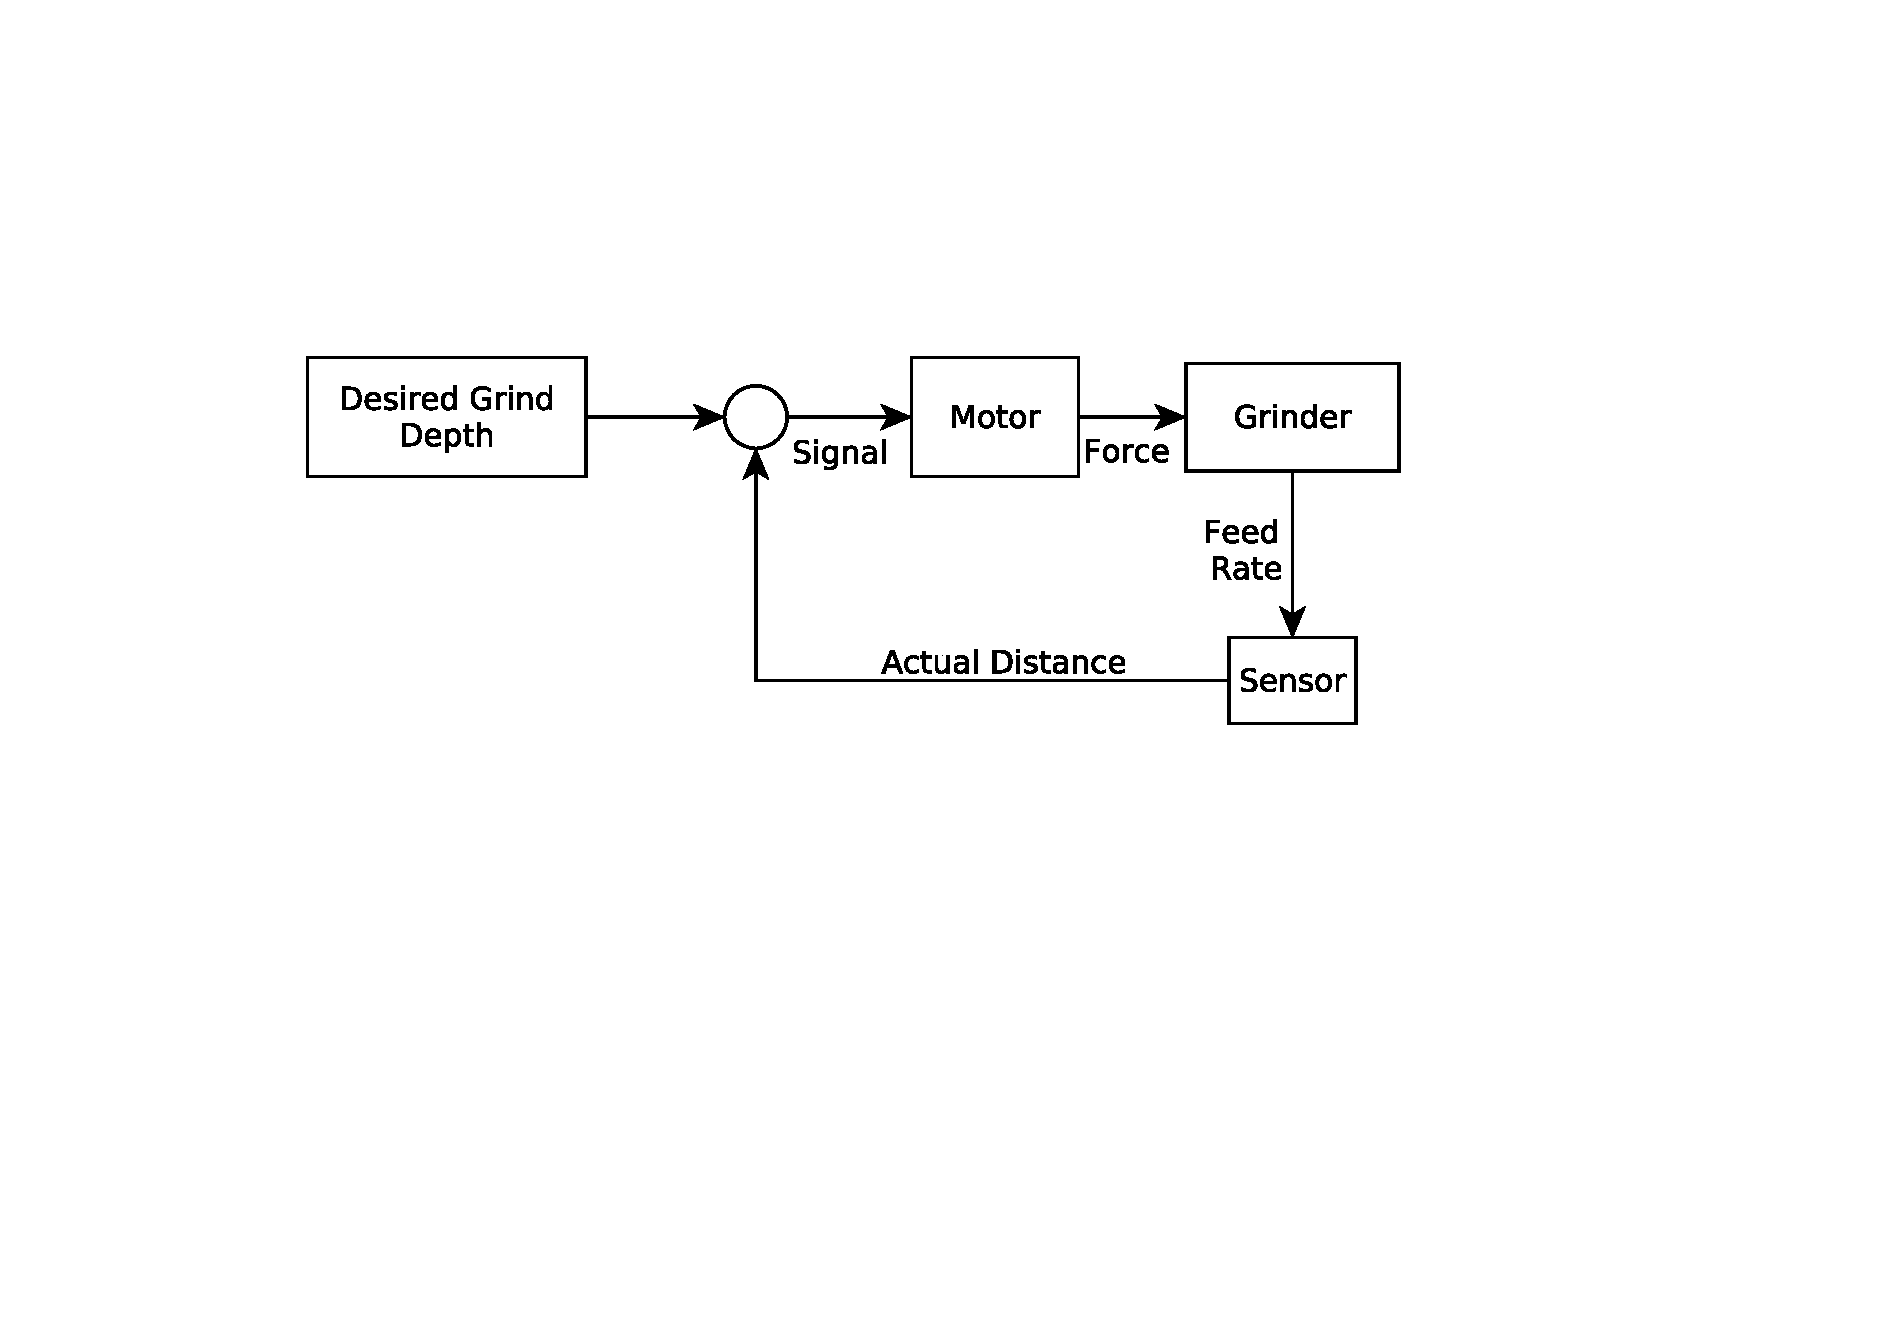
\includegraphics[width=\textwidth]{prob11}
		\end{minipage}

	\setcounter{enumi}{0}
	\item
		\begin{enumerate}
			%1.a
			\item 
				\begin{align*}
					\Lap{u(t)} 
					  &= \laplace{u(t)}
					\\&= \laplace{1}
					\\&= \inteval{\frac{1}{-s}\mathrm{e}^{-st}}{0}{\infty}
					\\&= \boxed{\frac{1}{s}}
				\end{align*}
			%1.b
			\item
				\begin{align*}
					\Lap{tu(t)} 
					  &= \laplace{tu(t)}
					\\&= \laplace{t}
					\\&= \frac{-t}{s}\e^{-st} - \int{\frac{-1}{s}\e^{-st}\ \del{t}}\ (\mathrm{integration\ by\ parts})
					\\&= \inteval{\frac{-t}{s}\e^{-st} - \frac{1}{s^2}\e^{-st}}{0}{\infty}
					\\&= \boxed{\frac{1}{s^2}}
				\end{align*}
			%1.c
			\item
				\begin{align*}
					\Lap{\sin{\omega t}\ u(t)} 
						  &= \laplace{\sin{\omega t} \cdot 1}
						\\&= \inteval{\frac{\e^{-st}}{s^2+\omega^2}(-s\sin{\omega t} - \omega\cos{\omega t})}{0}{\infty} \mathrm{(using\ integration\ table)}
						\\&= 0 - \frac{\e^0}{s^2+\omega^2}(0 - \omega)
						\\&= \boxed{\frac{\omega}{s^2+\omega^2}}
				\end{align*}
			%1.d
			\item
				\begin{align*}
					\Lap{\cos{\omega t}\ u(t)} 
					  &= \laplace{\cos{\omega t} \cdot 1}
					\\&= \inteval{\frac{\e^{-st}}{s^2+\omega^2}(-s\cos{\omega t} + \omega\sin{\omega t})}{0}{\infty} \mathrm{(using\ integration\ table)}
					\\&= 0 - \frac{\e^0}{s^2+\omega^2}(-s + 0)
					\\&= \boxed{\frac{s}{s^2+\omega^2}}
				\end{align*}
		\end{enumerate}
	\item
		\begin{enumerate}
				%2.a
				\item 
					\begin{align*}
						\Lap{\e^{-at}f(t)} 
						  &= \Lap{f(t)}(s+a)
						\\&= \Lap{\sin{\omega t}\ u(t)}(s+a)
						\\&= \boxed{\frac{\omega}{(s+a)^2+\omega^2}}
					\end{align*}
				%2.b
				\item
					\begin{align*}
						\Lap{\e^{-at}f(t)}
						  &= \Lap{f(t)}(s+a)
						\\&= \Lap{\cos{\omega t}\ u(t)}(s+a)
						\\&= \boxed{\frac{(s+a)}{(s+a)^2+\omega^2}}
					\end{align*}
				%2.c
				\item
					\begin{align*}
						\Lap{t^n u(t)} 
						  &= \frac{n!}{s^n+1}
						\\&= \boxed{\frac{3!}{s^3+1}\ \mid\ n = 3}
					\end{align*}
		\end{enumerate}

	\item
		\begin{enumerate}
				%3.a
				\item
					\begin{align*}
						F(s) 
						\\&= \frac{20s+6}{(s+3)(s+7)(s+11)}
						\\&= 
								\begin{bmatrix*}
									a = \frac{-60+6}{(4)(8)} & b = \frac{-140+6}{(-4)(4)} & c= \frac{-220+6}{(-8)(-4)}
								\end{bmatrix*}
								\begin{bmatrix*}
									  (s+3)^{-1}
									\\(s+7)^{-1}
									\\(s+11)^{-1}
								\end{bmatrix*}
						\\\therefore \Lapinv{F(s)} 
						  &= a\Lapinv{\frac{1}{(s+3)}} + b\Lapinv{\frac{1}{(s+7)}} + c\Lapinv{\frac{1}{(s+11)}}
						\\&= \boxed{a\e^{-3t} + b\e^{-7t} + c\e^{-11t}}
					\end{align*}
				%3.b
				\item
					\begin{align*}
							F(s) 
						\\&= \frac{s+8}{(s+2)^2(s+1)(s+5)}
						\\&= 
							\begin{bmatrix*}
								a = \frac{-7}{4} & b = \frac{3}{-36} & c = \frac{6}{-3} & d = \frac{-66}{9}
							\end{bmatrix*}
							\begin{bmatrix*}
								  (s+1)^{-1}
								\\(s+5)^{-1}
								\\(s+2)^{-2}
								\\(s+1)^{-1}
							\end{bmatrix*}^{\dagger}
						\\\therefore \Lapinv{F(s)} 
						\\&= a\Lapinv{\frac{1}{s+1}} + b\Lapinv{\frac{1}{s+5}} + c\Lapinv{\frac{1}{(s+2)^2}} + d\Lapinv{\frac{1}{s+2}}
						\\&= \boxed{a\e^{-t} + b\e^{-5t} + ct\e^{-2t} + d\e^{-2t}}
					\end{align*}
					\begin{align*}
						^{\dagger}\ 
							  &\left. \mathrm{K}_i = \lim_{s \to -p_i} \frac{1}{(i-1)!} \mathcal{D}^{i-1}[F_i(s)]\ \right| 
								  F_i(s) = \frac{\mathrm{N}(s)}{\mathrm{D(s)}}(s-p_i)
							\\&\therefore d = \lim_{s \to -2} 1\cdot \mathcal{D}[\frac{s+8}{(s+1)(s+5)}] = \frac{-66}{9}
					\end{align*}
			\end{enumerate}

	\setcounter{enumi}{4}
	%5.a
	\item
		\begin{enumerate}
			\item
				\begin{align*}
					  &\Lap{5t^2\cos{(3t+45)}} =
					% imported from matlab
					\\& 5\, \sin\!\left(45\right)\, \left(\frac{6}{{\left(s^2 + 9\right)}^2} - \frac{24\, s^2}{{\left(s^2 + 9\right)}^3}\right) - 5\, \cos\!\left(45\right)\, \left(\frac{6\, s}{{\left(s^2 + 9\right)}^2} - \frac{8\, s^3}{{\left(s^2 + 9\right)}^3}\right)
				\end{align*}
			\item
				\begin{align*}
					  &\Lap{5t\e^{-2t}\sin{(4t+60)}} =
					% imported from matlab
					\\& \frac{20\, \cos\!\left(60\right)\, \left(2\, s + 4\right)}{{\left({\left(s + 2\right)}^2 + 16\right)}^2} - 5\, \sin\!\left(60\right)\, \left(\frac{1}{{\left(s + 2\right)}^2 + 16} - \frac{\left(2\, s + 4\right)\, \left(s + 2\right)}{{\left({\left(s + 2\right)}^2 + 16\right)}^2}\right)
				\end{align*}
		\end{enumerate}

	\item
		\begin{enumerate}
			\item
				\begin{align*}
					  & \Lapinv{\frac{(s^2+3s+7)(s+2)}{(s+3)(s+4)(s^2+2s+100)}} =
					% imported from matlab
					\\& 2107\, \delta\!\left(t\right) - 721\, \mathrm{e}^{- 3\, t} + 1535\, \delta^{(1)}\!\left(t\right) + 651\, \delta^{(2)}\!\left(t\right) + 127\, \delta^{(3)}\!\left(t\right) + 8\, \delta^{(4)}\!\left(t\right) + \delta^{(5)}\!\left(t\right)
				\end{align*}
			\item
				\begin{align*}
					  & \Lapinv{\frac{s^3+4s^2+6s+5}{(s+8)(s^2+8s+3)(s^2+5s+7)}} = 
					% imported from matlab
					\\& \frac{1073\, \mathrm{e}^{- 4\, t}\, \left(\cosh\!\left(\sqrt{13}\, t\right) - \frac{127\, \sqrt{13}\, \sinh\!\left(\sqrt{13}\, t\right)}{481}\right)}{417} - \frac{239\, \mathrm{e}^{- 8\, t}}{93} - \frac{14\, \mathrm{e}^{-\frac{5\, t}{2}}\, \left(\cos\!\left(\frac{\sqrt{3}\, t}{2}\right) + \frac{1907\, \sqrt{3}\, \sin\!\left(\frac{\sqrt{3}\, t}{2}\right)}{21}\right)}{4309}
				\end{align*}
		\end{enumerate}

\end{enumerate}

\end{document}
